\documentclass[journal]{IEEEtran}

% *** GRAPHICS RELATED PACKAGES ***
%
\ifCLASSINFOpdf
  % \usepackage[pdftex]{graphicx}
  % declare the path(s) where your graphic files are
  % \graphicspath{{../pdf/}{../jpeg/}}
  % and their extensions so you won't have to specify these with
  % every instance of \includegraphics
  % \DeclareGraphicsExtensions{.pdf,.jpeg,.png}
\else
  % or other class option (dvipsone, dvipdf, if not using dvips). graphicx
  % will default to the driver specified in the system graphics.cfg if no
  % driver is specified.
  % \usepackage[dvips]{graphicx}
  % declare the path(s) where your graphic files are
  % \graphicspath{{../eps/}}
  % and their extensions so you won't have to specify these with
  % every instance of \includegraphics
  % \DeclareGraphicsExtensions{.eps}
\fi


\usepackage{amssymb}
\usepackage{graphicx}
\usepackage{multirow}
\usepackage{amsmath}
\usepackage{siunitx}
\usepackage{url}
% correct bad hyphenation here
\hyphenation{op-tical net-works semi-conduc-tor}


\begin{document}
%
% paper title
% Titles are generally capitalized except for words such as a, an, and, as,
% at, but, by, for, in, nor, of, on, or, the, to and up, which are usually
% not capitalized unless they are the first or last word of the title.
% Linebreaks \\ can be used within to get better formatting as desired.
% Do not put math or special symbols in the title.
\title{Network-based Online Video freeze prediction in HTTP Adaptive Streaming}
%
%
% author names and IEEE memberships
% note positions of commas and nonbreaking spaces ( ~ ) LaTeX will not break
% a structure at a ~ so this keeps an author's name from being broken across
% two lines.
% use \thanks{} to gain access to the first footnote area
% a separate \thanks must be used for each paragraph as LaTeX2e's \thanks
% was not built to handle multiple paragraphs
%

\author{Tingyao~Wu,~\IEEEmembership{Member,~IEEE,}
				Stefano~Petrangeli,~\IEEEmembership{Member,~IEEE,}
        Rafael~Huysegems,~\IEEEmembership{Member,~IEEE,}
        and~Tom~Bostoen,~\IEEEmembership{Life~Fellow,~IEEE}% <-this % stops a space
\thanks{T. Wu, R. Huysegems and T. Bostoen are with Bell Labs, Alcatel-Lucent, Copernicuslaan 50, B-2018 Antwerpen, Belgium. e-mail: (tingyao.wu@alcatel-lucent.com).}% <-this % stops a space
\thanks{S. Petrangeli is with Department of Information
Technology (INTEC), Ghent University- iMinds, Gaston Crommenlaan
8 (Bus 201), 9050 Ghent, Belgium.}% <-this % stops a space
\thanks{Manuscript received April 19, 2005; revised September 17, 2014.}}

% note the % following the last \IEEEmembership and also \thanks - 
% these prevent an unwanted space from occurring between the last author name
% and the end of the author line. i.e., if you had this:
% 
% \author{....lastname \thanks{...} \thanks{...} }
%                     ^------------^------------^----Do not want these spaces!
%
% a space would be appended to the last name and could cause every name on that
% line to be shifted left slightly. This is one of those "LaTeX things". For
% instance, "\textbf{A} \textbf{B}" will typeset as "A B" not "AB". To get
% "AB" then you have to do: "\textbf{A}\textbf{B}"
% \thanks is no different in this regard, so shield the last } of each \thanks
% that ends a line with a % and do not let a space in before the next \thanks.
% Spaces after \IEEEmembership other than the last one are OK (and needed) as
% you are supposed to have spaces between the names. For what it is worth,
% this is a minor point as most people would not even notice if the said evil
% space somehow managed to creep in.



% The paper headers
\markboth{Journal of \LaTeX\ Class Files,~Vol.~13, No.~9, September~2014}%
{Shell \MakeLowercase{\textit{et al.}}: Bare Demo of IEEEtran.cls for Journals}
% The only time the second header will appear is for the odd numbered pages
% after the title page when using the twoside option.
% 
% *** Note that you probably will NOT want to include the author's ***
% *** name in the headers of peer review papers.                   ***
% You can use \ifCLASSOPTIONpeerreview for conditional compilation here if
% you desire.




% If you want to put a publisher's ID mark on the page you can do it like
% this:
%\IEEEpubid{0000--0000/00\$00.00~\copyright~2014 IEEE}
% Remember, if you use this you must call \IEEEpubidadjcol in the second
% column for its text to clear the IEEEpubid mark.



% use for special paper notices
%\IEEEspecialpapernotice{(Invited Paper)}




% make the title area
\maketitle

% As a general rule, do not put math, special symbols or citations
% in the abstract or keywords.
\begin{abstract}
HTTP adaptive streaming (HAS) has become a prevailing technology for media delivery technology over mobile and fixed networks. 
%Internet service providers and CDN (Content Delivery Network) providers are interested in network-based monitoring the client's Quality of Experience (QoE) for HAS video sessions. 
The client's Quality of Experience (QoE) for HAS video sessions is particularly of interests in network providers and Content Delivery Network (CDN) providers. But typically, network providers are not able to assess to clients to obtain QoE relevant parameters, such as freeze, initial loading time, quality switches, etc.
 
In our previous work, we designed a HAS QoE monitoring system based on the sequence of HTTP GET requests collected at the CDN nodes. The system relies on a technique called session reconstruction to retrieve the major QoE parameters without modification of the clients. However, session reconstruction is computationally intensive and requires manual configuration of reconstruction rules. 
To overcome the limitations of session reconstruction, this paper proposes a scalable machine learning (ML) based scheme that detects video freezes using a few high-level features extracted from the network-based monitoring data. 
We determine the discriminative features for session representation and assess five potential classifiers. We select the C4.5 decision tree as classifier because of its simplicity, scalability, accuracy, and explainability. To evaluate our solution, we use traces of Apple HTTP Live Streaming video sessions obtained from a number of operational CDN nodes and traces of Microsoft Smooth Streaming video sessions acquired in a controlled lab environment. Experimental results show that an accuracy of about 98\%, 98\%, and 90\% can be obtained for the detection of a video freeze, a long video freeze, and multiple video freezes, respectively. Excluding log parsing, the computational cost of the proposed video-freeze detection is 33 times smaller than needed for session reconstruction.

\end{abstract}

% Note that keywords are not normally used for peerreview papers.
\begin{IEEEkeywords}
HTTP Adaptive Streaming, Decision Tree C4.5, Freeze Prediction, Quality of Experience
\end{IEEEkeywords}






% For peer review papers, you can put extra information on the cover
% page as needed:
% \ifCLASSOPTIONpeerreview
% \begin{center} \bfseries EDICS Category: 3-BBND \end{center}
% \fi
%
% For peerreview papers, this IEEEtran command inserts a page break and
% creates the second title. It will be ignored for other modes.
\IEEEpeerreviewmaketitle



\section{Introduction}
\label{sec:intro}
% The very first letter is a 2 line initial drop letter followed
% by the rest of the first word in caps.
% 
% form to use if the first word consists of a single letter:
% \IEEEPARstart{A}{demo} file is ....
% 
% form to use if you need the single drop letter followed by
% normal text (unknown if ever used by IEEE):
% \IEEEPARstart{A}{}demo file is ....
% 
% Some journals put the first two words in caps:
% \IEEEPARstart{T}{his demo} file is ....
% 
% Here we have the typical use of a "T" for an initial drop letter
% and "HIS" in caps to complete the first word.
\IEEEPARstart{V}{ideo} streaming has occupied more than half of traffic over the Internet. In recent years, video delivery over traditional best-effort Internet becomes very popular. Among this, HTTP Adaptives Steaming (HAS) is increasingly adopted and has become a key technology. HTTP adaptive streaming systems~\cite{stockhammer2011dynamic} include MPEG-DASH, Apple's HTTP Live Streaming, Microsoft’s Smooth Streaming, Adobe’s Dynamic Streaming, etc. Typically, in a HAS architecture, video content, hosted on an HTTP Web server, is encoded in different quality levels (bit-rates), and chunked into independent segments. A HAS client requests the segments with different qualities in a linear way using HTTP GET requests and downloads them using plain HTTP progressive download. The retrieved segments can be played back as a seamless video, possibly switching among different quality levels. The key feature of HAS is that it is the client that is responsible for determining which quality level to download according to its available resources. Server/network providers do not have the control over the quality requests.  
One of the main advantages of introducing HAS as a delivery/playout method is that, the client could adapt its quality requests based on the perceived bandwidth: it enables the client to smoothly play the video with a low quality level even when the perceived bandwidth is very limited, while when a high bandwidth is available, it supports the client to demand high quality levels.  

With the growing pervasion of HAS deployments, network and CDN providers raise interests in knowing the end-user quality of experience (QoE) of HAS sessions over their network, because the user-centric QoE reveals the satisfaction of their users. Although QoE is the subjective perception of end-users, the objective QoE relevant parameters, including the statistics of bit-rates, freezes frequency and freeze durations, etc, can be used to model the end-users' Mean Opinion Score (MOS)~\cite{de2013model}. This inspires network/CDN providers to obtain the QoE relevant parameters, as an indirect way to evaluate the satisfaction of end-users. While a HAS client may report these parameters to the Web server (for instance, enabling Advanced Logging in Microsoft Internet Information Services (IIS) could require Microsoft Silverlight clients to send the status of medie content consumption to the IIS server at a regular time basis), typically it does not report these parameters to intermediate network nodes; they are only able to intercept the sequence of HTTP GET requests sent from the client to the server/CDN. So retrieving QoE relevant parameters from the sequence of HTTP GET requests within a single video session is a plausible method to evaluate end-user's QoE. 
Indeed, in our previous study~\cite{huysegems2012session}, we demonstrated that from the sequence of HTTP GET requests collected at intermediate network elements, the HAS session can be reconstructed to derive all QoE related parameters. These parameters include the average playout quality, changes in the play-out quality, rebuffering due to buffer starvation, rebuffering caused by interactivity, etc. The session reconstruction technique relies on some manually rules discovered by the trial-and-error method, without modifying the original HAS client, and thus is a feasible network based method to evaluate the video delivery quality of HAS.

Among all objective QoE relevant metrics, freeze/re-buffering is undoubtedly the most deleterious factor to destroy end-users' satisfaction and engagement. The 2015 annual report of Conviva~\cite{convivaC:2015} shows that 28.8\% of video sessions experience at least one rebuffering event, but only 1\% increase of rebuffering could reduce the video engagement with 14 minutes. Identifying freeze/rebuffering events is thus the primary task for retrieving the QoE relevant metrics. Although the session reconstruction in our previous work has shown its effectiveness, the manual effort of the trial-and-error rule exploration reduces its generalization capability; one has to manually re-configure the construction rules for a new HAS deployment. Meanwhile, for about 70\% buffering-free video sessions, such {\it no-freeze} information is not known until a session has been fully reconstructed. Since session reconstruction needs a time-consuming segment-by-segment alignment, it is more desirable to have a quick method to identify whether a video session contains freeze(s) before taking session reconstruction. This inspires us to develop a scalable freeze detection/prediction technique at the intermediate network node for a video session, ideally without the requirement of any deployment-dependent reconstruction rules. In fact, in~\cite{wu:iwqos15}, we have demonstrated the concept of using a decision tree-based freeze detection technique to retrieve the freeze information for a full video session with a high accuracy, whereof this paper represents an extension.

The main contributions of this paper are two-fold. First, we investigate a few feasible machine learning techniques and select C4.5 decision tree as our classifier. The selection compromise the computational cost, simplicity, stability and understandability. Second, as the extension of our work in~\cite{wu:iwqos15}, which assumes that there is no user interactivity, we examine the performance of the proposed method in the existence of user interactivity, including pause and re-positioning. Third, the approach is transplanted into an OpenFlow-based framework to help clients avoiding video freezes under limited bandwidth conditions. In this scenario, the approach is used to online predict whether the normal delivery of a video segment could lead to a freeze at the client side in a near future; if a potential freeze is foreseen, a priority to the current segment is given to avoid the true occurrence of the freeze. 

The remainder of this paper is organized as follows. Section~\ref{sec:related_work} gives the overview of the research of HAS QoE and the introductin of OpenFlow. Section~\ref{sec:framework} presents the proposed freeze detection/prediction framework, while in section~\ref{sec:exp} we demonstrate the designed experments and the corresponding results. The conclusions and future work are presented in section~\ref{sec:conclusions}.


\section {Related work}
\label{sec:related_work}
\subsection{QoE in HTTP Adaptive Streaming}

Quality of Experience (QoE) is a user-perceived metric that describes the the degree of satisfaction of the user of an application or service. In video service, the subjective user test is the golden rule metric measurement for the QoE. %In the evaluation of HAS based QoE, the subjective perception to the video service is also widely adopted. 
The subjective perception test can be easily influenced by the human psychological factor and by the bias of user interests. Moreover, it is typically a time-comsuming and expensive procedure. Thus some intrinsic quality metrics, including Peak Signal to Noise Ratio (PSNR), Structural Similarity (SSIM), and Video Quality Metric (VQM), are taken into account in traditional video QoE analysis, attempting to map these metrics to the degree of human satisfaction. 

Lately, the HAS based QoE research has already received a lot attention. As HAS could adapt to different network enviroments by increasing/decreasing quality levels and also by filling/depleting the buffer filling level, it could mitigate the freeze occurrences. Thus it is considered to be an effective technique to enhance the end-user's QoE. On the contrary, the reaction of classial HTTP video streaming (e.g. progressive downloading) to fluctuating network conditions only relies on the changing of buffer level. ~\cite{yitong2013study} studies the QoE of DASH in comparison with fixed-bitrate streaming and gives the evidence that adaptive streaming improves end-users' subjective perception greatly compared with fixed-rate streaming in terms of QoE. This advantage is also verified in~\cite{yao2011empirical}, which compares adaptive and fixed-rate streaming under vehicular mobility circunstance and reveals that HAS can effectively reduce freeze by 80\% when bandwidth decreases, could better utilize the available bandwidth when bandwidth increases.

Comparing to traditional video delivery technique, the HAS extends single quality level to mutliple quality levels with respective to resolution. This extended dimension introduce a new factor, changing video quality levels (i.e., adaptation) and thus has new impacts on QoE. In fact, traditional quality metrics (PSNR, SSIM and VQM, etc) fail to predict user-perceived video quality due to quality fluctuations inherent to HAS systems~\cite{lievens2015perceptual}. Instead, the playback start time, number of freezes, duration of freezes, ratio of freezes, quality levels (together with their first order and second order statistics), bitrate switching frequency, etc are the objective representives~\cite{julurimeasurement} that are able to capture the factors that influence the user's QoE in HAS system. In~\cite{garciaquality}, the authors overview the recent studies targeting the optimization of HAS adaptation strategy, concerning subjective evaluation of HAS QoE, and also highlight the challenges and open research questions related to QoE assessment in HAS. Seufert et al.~\cite{seufertsurvey} provides a comprehensive survey for the relationship of HAS and subjectively perceived quality. In the survey, the main influence factors of QoE of HTTP video streaming are discussed, and the influence of temporal resolution, spatial resolution and video quality on QoE are also presented.

\subsection{Freeze reduction in HAS client}
Almost all research agree that video freeze sharply degrades the QoE. Freeze, also called stalling/interruption/buffer-underruning, etc in the literature, is the stopping of video playback because of the depletion of playout buffer. This typically happens when the received video segment in time is continuously lower than the speed of playback, leading to the decreasing of buffer filling level at the client. Eventually, insufficient data is available in the buffer and the playback of the video has to stop. The playback continues when a certain amount of video data is received again. Freeze is a sudden unexpected interruption during watching. This unexpectation is probably processed differently by the human sensory system, and degrades the users' satisfaction~\cite{sackl2013evaluating}. 

By nature, HAS is designed to reduce freeze in volatile network situation. However, as the increasing demand of high quality videos, it is unavoidable to experience the occurrence of freeze during HAS video playout, especially when a sudden bandwidth drop occurs~\cite{akhshabi2012experimental,riiser2012comparison}. There have been quite a few studies concerning further reducing the occurrence of freezes in HAS by elaborately designing the client rate adaptation heuristic. For instance, ~\cite{claeys2014design} and ~\cite{wu2014factor} use the reinforcement learning technique as a decision agent at the HAS client. The agent learns to request the most suitable quality level given the client's instant status by progressively optimizing the QoE-related reward. In the design, the punishment to a freeze is about 2 order of magnitude than low qualities and quality switching. In ~\cite{liu2011rate}, a rate adaptation algorithm for HAS was proposed to detect bandwidth changes using a smoothed HTTP throughput measure based on the segment fetch time. It deploys a step-wise increase/aggressive decrease method to switch up/down between the different quality levels to prevent from the freeze that might be incurred by sudden bandwidth drops. In ~\cite{huang2013downton, huang2014using}, the authors argue that only observing and controlling the playback buffer, without having to take network capacity into account, is already able to avoid unnecessary rebuffering and control the delivered video quality. 

\subsection{Network based freeze reduction/discovery}
In-network HAS QoE monitoring provides a solution for network/CDN providers to reveal how end-user is satisfied with the video service. ~\cite{huysegems2012session} demonstrates a session reconstruction technique lying at an intermediate node to fully recover how the media content was consumed at the client. The technique could reconstruct the place and duration of the occurence of freeze, and the pause and re-positioning initiated by the end-users, using the sequence of intercepted HTTP GET messages sent by the client to the server. By the session reconstruction, all QoE metrics can be retrieved. However, this technique relies on manual effort to define some heurisitc dependent rules thus it has scalability issues when dealing with newly emerged HAS clients.

To reduce the impact of freeze and optimize the QoE for multiple clients, some researchers also seek for in-network solutions for HAS. In~\cite{bouten2012qoe, bouten2015qoe} presents merits of deploying intelligent network elements that manage the QoE in HAS delivery network. It was argued that a combination of HAS enabled clients with the operator-centric of user-centric policy enforced at the intelligent proxies leads to the best solution. 
~\cite{Petrangeli:qcman15} presents an interesting OpenFlow-based framework, in which an in-network controller is in charge of introducing prioritized delivery of HAS segments based on status collected from both the network nodes and the HAS clients. Once a HAS client is approaching buffer-underrun, the prioritization mechanism at the controller is triggered for the client, then the requested segment (and possibly the next few segments) will be delivered to the client with a high priority, in order to avoid the potential freeze really happening. However, as we stated in the section~\ref{sec:intro}, in reality, the network node usually is not able to acquire the report from the client. Moreover, the system could be attacked by a malicious client who transmit incorrect information to take advantage of the prioritization. Thus a pure in-network solution is more desirable.



\section{In-network freeze detection/prediction}
\label{sec:framework}
In this section, we detail our approach of detecting/predicting freeze for HAS video sessions from the perspective of an intermediate node. As freeze is the most influential factor to impact the end user's QoE, the network/CDN providers could use this knowledge to actively manage, monitor or enhance the QoE in their network in general. Macroscopically, aggregated HAS QoE metrics for different sessions provides a good view on the occupation of the network. For example, a low average viewing quality and frequent freezing occurences could be a sign of the neccesity of enlarging the bandwidth with certain network nodes for the operator. Microscopically, the network provider could faciliate the output of the online in-network freeze prediction: without the feedback from the client, the provider can decide if a prioritization is necceary assign higher priority traffic class when the play-out buffer at the client is close to an underrun, thereby actively preventing a likely rebuffering event for that HAS client.

\subsection{Architectural description}
Figure~\ref{fig:positioning} illustrates the utility and position of the proposed network-based video freeze detection/prediction in the CDN loop. The network topology is composed of original HAS server, CDN and HAS client, together with a {\it priority controller} module~\cite{Petrangeli:qcman15} adhered to the CDN. This module behaves the interface for the task of freeze prediction. The CDN node maintains a log file tracking all segment-level HTTP requests from multiple clients' HAS video sessions. The log file is parsed through the {\it session log parsing} block, and is split into multiple session logs, each containing all HTTP requests for one single video session. The session separation is done by examining the unique MD5 of a session embedded in each of HTTP request. The feature extraction module is used to extract a few attributes either for a video session in the task of freeze detection, or for a segment request in the task of freeze prediction. In the training phase, the status report of the HAS client, called groundtruth, is required for both tasks, in order to train the detection/prediction classifers in a supervised mode. The status report includes, if applicable, the knowledge of the occurred user interactivies and the experienced freezes.

\subsubsection{Session-level freeze detection}
The session-level freeze detection aims at quickly providing moderately in-depth knowledge of freeze in a video session. The knowledge of freeze includes: (a) Does the concnerned video session contain any freeze? (b) Is the longest freeze, if exists, longer than a threshold, e.g. 10 seconds? (c) Are there multiple freezes in the session? The yes/no binary answers to the above three questions in fact are three binary classification tasks. Note that the answers give a general idea of the rebuffering, but do not reveal the details, e.g. the position and the exact duration of freezes. On the other hand, the scalable expenditure of computational cost is another concerned issue. According to~\cite{convivaC:2015}, around 70\% of video sessions do not contain any freeze. Usually there are ten of thousands of concurrent video sessions delivered by a CDN node. Thus it is desired to quickly focus on problemic sessions. Therefore, in the freeze detection, we focus on session-level classification.

In the training step, all individual training sessions are tracked and separated from the CDN log. A feature vector is then extracted to represent the high level information of a single video session. In the meanwhile, the groundtruth, containing is collected from the corresponding client. The feature vectors and the groundtruth are coupled in the {\it training} module. Then three classifiers in terms of the above three questions are built. In the test, a testing feature vector for a testing video session is classified by the three binary classifiers. The combined recognized results represent the freeze status of the testing session.
  
\subsubsection{Segment-level freeze prediction}
The in-network segment-level freeze prediction is an online process. It attempts to forecast whether a freeze is approaching at the client when a request is received and the requested segment is about to deliver to the client from the CDN. If the prediction result gives an indication that the client is experiencing a freeze or will have a freeze shortly, the {\it priority controller}, as described in~\cite{Petrangeli:qcman15}, will assign a priority-delivery note to this segment. The segment will be delivered with a higher priority, to rescue the client from freeze, or to avoid the freeze really happening.

In the training, the feature vector is extracted for each single segment request. The true label of a feature vector would be the event that happens at the client in between the time that the current and the next segment are about to be delivered. All feature vectors and their labels are trained in a supervised way to generate a prediction classifier. In the test phase, when the {\it priority controller} is going to deliver a segment to the client, it will inquiry the prediction classifier to check whether there is a high risk that the client is close to freeze. If the prediction result is no, then the segment is delivered as the usual way. Otherwise, the priority will be given to the segment. 

%These video sessions are the input of the freeze detection, as shown in the dashed box in Figure~\ref{fig:positioning}. There are two main modules in this study, namely modeling and detection respectively, which will be further explained in section~\ref{subsec:system_description}. The output of the freeze detection is the rebuffering information of a single video session. If a session does not contain any freeze, then its global QoE rating can be achieved by combining with other QoE parameters (such as quality). If a session is identified as having a freeze, having at least one long freeze or having multiple freezes, this session is optionally sent to the HAS session reconstruction~\cite{huysegems2012session} module to obtain the detailed freeze-information

\begin{figure}[!t]
\begin{center}
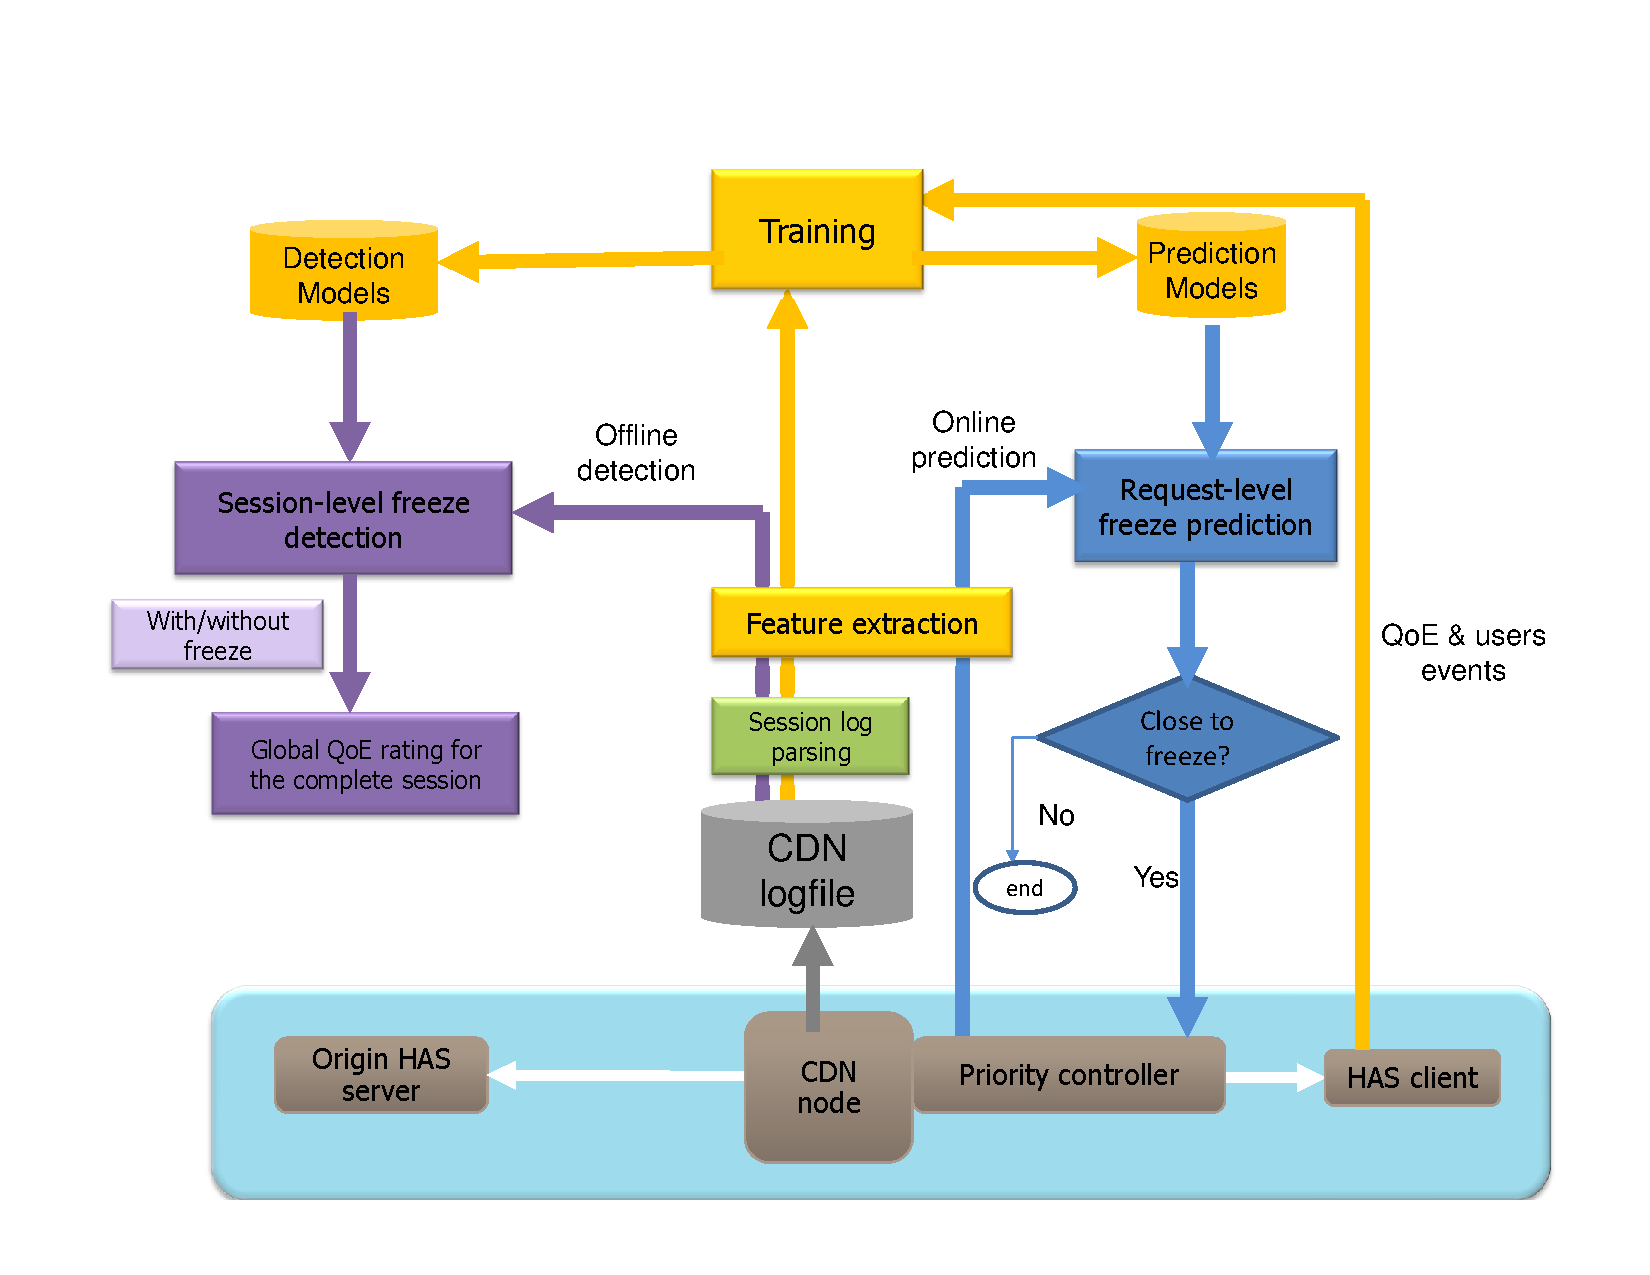
\includegraphics[width=90mm] {graphs/positioning.pdf}
\caption{Position of freeze detection/prediction in the CDN loop}
\label{fig:positioning}
\end{center}
\end{figure}

\section{Methodology}

\subsection{Problem statement}
From the machine learning point of view, the freeze detection/prediction is to look for a mapping function between the sequence of HTTP GET messages for a single video session from either an origin server or a CDN node with the occurrence of freezes at the client. A few disturbances may reduce the mapping accuracy. 
\begin{itemize}
\item {Segment retrieval}. There is no guarantee that the client can successfully receive the segment in time. Due to certain reasons, for example traffic congestion, the client may not receive the segment, which is unknown for the network provider. 
\item{Unknow status and heuristic-dependent parameters}
The sequence of HTTP GET requests does not reveal the instant status of the heuristic (such as the remaining buffer filling level and the perceived bandwidth) and the intrinsic heuristic-dependent parameters (including the segment length, the maximum buffer size, the initial startup delay, etc). 
\item{User Interactivity}. Some interactive operations taken by end-users could be difficult to be detected. For instance, in the video-on-demand (VOD) scenario, when the end-user pauses the playout, there are two different behaviors with repective to the segment requests: if the client is in the loading state (the state in which the client wants to fill the buffer as quickly as possible), it will keep asking new segments to fulfill the buffer, until the maximum buffer size is reached; but if the client is already in the steady state when pause , it does not send any requests. In this case, the network node does not receive any requests as well, and may conjecture that the client has already been experiencing a long freeze. 
\end{itemize}
%Fourth, the client maintains a buffer which guarantees the smooth playout. Typically when a client is playing a segment, it already starts to ask for a segment in a few seconds.  

%, which from the network sideobservations of HTTP GET requests at the CDN side. (especially pause). CDN providers have to infer how delivered video segments are consumed based on the requests in the log files. If a server/CDN node receives requests with a fixed time interval between segments approximately equal to the duration of a segment, it probably means that the client-buffer is completely filled and the playback is currently free of freezes; if the requests are received close after each other, it may indicate the client is in loading state (the state in which the client wants to fill the buffer as quickly as possible) or in panic state (the state in which the client buffer is close to an under-run). If the time interval of consecutive requests is much longer than the segment duration, there is a high probability that the client is experiencing a freeze. To identify based on network/CDN logs whether rebuffering events occurred at the client side, we rely on machine learning techniques.

%
%\begin{table}[th]
%\begin{center}
%\caption{Mathematical denotion}
%\begin{tabular}{cc|cc|}
%\hline\hline
%
%\hline
%$s\in{\mathbf{S}}$									& session $s$ in the training set $\mathbf{S}$			& $L$								& segment length in seconds\\
%$t_i$																& timestamp for receiving $i$ segment request				& $q_i$							& the quality level of segment $i$  \\ 
%$I_i$																& inter-segment duration $$I_i=t_{i+1}-t_{i}$$					& $d_{ki}$					& average inter-segment durations
%
%\hline
%\hline
%$Mean(I)$ & 0.50 & $Mean(I)$ & 0.42 & $Mean(I)$ & 0.25 \\
%$Median(I)$ & 0.09 & $Median(I)$& 0.06 & $Median(I)$ & 0.07 \\
%\hline\hline
%\end{tabular}
%\label{tab:feature_ranking_hls}
%\end{center}
%\end{table} 

A sequence of HTTP GET messages for a video session $s$ ($s\in{\mathbf{S}}$, where $\mathbf{S}$ is the set of video sessions) typically contain the timestamp $T(s)=\{t_i^s, 1\leq{i}\leq{N_s}\}$ that the message is received and the requested quality level $Q(s)=\{q_i^s, 1\leq{i}\leq{N_s}\}$, where $N_s$ is the number of segments in the session $s$. The inter-segment duration $I_i^s$ between segment $i$ and segment $i+1$ is defined as $I_i^s=t_{i+1}^s-t{i}^s$. Then for a session $s$, the useful information related to freeze directly obtained from HTTP GET messages can be represented as $M(s)=\{T(s),Q(s)\}$.

In the training step, from the client groundtruth of session $s$, we know exactly the freeze related segment-level event happened between $t_i^s$ and $t_{i+1}^s$. The event $e_i^s$, ($0\leq{e_i^s}<I_i^s$) is the duration of freeze in this period; if there is no freeze, then $e_i^s=0$. The $e_i^s=0$ indeed is the true label in the task of freeze prediction. Moreover, from $E(s)=\{e_i^s,1\leq{i}\leq{N_s}-1\}$, we can obtain the session level labels $YF(s)$, $YL(s)$ and $YM(s)$ for session $s$, in which $YF(s)$ is the binary label for the existence of freeze, $YL(s)$ is the label for the exitence of long freeze, and $YM(s)$ represents the multi-freeze information:
\begin{equation}
YF(s) =
  \begin{cases}
    1       & \exists{j},\quad e_j^s>0 \\
    0  		& otherwise\\
  \end{cases}
\end{equation}

\begin{equation}
YL(s) =
  \begin{cases}
    1       & \exists{j}, \quad e_j^s>F \\
    0  		& otherwise\\     
  \end{cases}
\end{equation}

\begin{equation}
YM(s) =
  \begin{cases}
    1       & \exists{i,j},\quad i\neq{j},  \quad e_j^s>0\cap{e_i^s>0} \\
    0  		& otherwise\\
  \end{cases}
\end{equation}
$F$ is an arbitrary threshold for long freeze, for instance, 10 seconds.
                                                                                   
The task of freeze detection/prediction is to learn a function $g:\mathfrak{X}\to\mathfrak{Y}$. The instance $\mathbf{x}\in\mathfrak{X}$ is a feature vector extracted from the original sequence of HTTP GET requests. Depending on various tasks, the procedure of feature extraction is slightly different (see section~\ref{subsec:feature_extraction}). 
%The label $y\in\mathfrak{Y}$ is the combination of $T(s)$ and $Q(s)$, and a label $y(s)\in\mathfrak{Y}$ can be $YF(s)$, $YL(s)$ and $YM(s)$. For the task of freeze prediction, the input instance $\mathbf(x)$ contains the temporal information: a function $h$ is learned to map the segment-level information to the label: $h:\mathfrak{X}\to\mathfrak{Y}$, where an input instance $\mathbf{x}$ in $\mathfrak{X}$ $=\{I_k^s,q_k^s\}$, and $\mathfrak{Y}={e_i^s}$, where


\subsection{Assumption}
A few prerequisites are assumed in this study. First, as we are investigating video picture freeze, the requests of audio segments are ignored, unless otherwise stated. Apparently, the discontinous audio could impact the end user's QoE. But because the byte size of audio segments is usually much smaller than that of video segments (even the lowest quality level), the delivery is less likely to be the reason of audio discontinuity. Second, user interactivity behaviors are restricted to pause/play and forward/backward jump. Typically, there are six types of user interactions with a video player: play, pause, forward, rewind, jump and stop. Forward/rewind can be seens as a special case of jump, and stop is the end of video playout. So forward/rewind and stop are not treated seperately in the study of freeze detection/prediction with user interactivity. Third, we do not consider caching between the delivery node and the video player; all segment requests are received by the CDN/network node. Actually, the impact of caching in HAS is not well studied~\cite{lee2014caching}. Intuitively, multiple quality levels for the same video segment in HAS reduces the efficiency of a cache. In practise, from the observation of {\it field dataset} (see section~\ref{subsubsec:field_data_set}), the caching operation only happens very few times, if any. Last, we assume the fixed segment length for a given HAS heuristic. Although there have been some studies related to adaptive segment length~\cite{adzic2012optimizing, lievens2013optimized}, the mainstream manufactures still take the fixed segment length as standard. 

\subsection{Feature extraction and classifier selection}
\label{subsec:feature_extraction}
\subsection{Estimate of In-heuristic parameters}
Some heuristic-dependent parameters can be empirically estimated from the training set before the learning process. Generally segment duration $L$, initial delay $u$ and maximum buffer size in seconds $M$ are three important parameters to determine the whole playout procedure. But these parameters are usually unknown for a network provider. In this subsection, without lossing generality, we ignore the session notion $s$.

\subsubsection{Segment length}
The precise segment duration $L$ is crucial for buffer filling estimation. One way to obtain the segment duration is to intercept and parse the manifest file at the CDN, which is an extra effort. The other way is to use the property of HAS itself: in a freeze-free session, a segment cannot be requested too early, due to the limitation of the maximum buffer length; the segment cannot be retrieved too late either because the late arrival could result in a freeze. Denote the initial delay is $u$ seconds, the maximum buffer limit is $M$ seconds ($M>u$), and the number of segments in a session is $N$, then for a session without any freeze, the last segment must be fully obtained between $N\times{L}-M+u$ and $N\times{L}+u$, to guarantee a freeze-free session: 
$N\times{L}-M+u<\sum{I_i}<N\times{L}+u$, 
leading to $\frac{\sum{I_i}}{N}-\frac{u}{N}<L<\frac{\sum{I_i}}{N}-\frac{u-M}{N}$. 
When $N\rightarrow{+\infty}$, $L\approx{\frac{\sum{I_i}}{N}}$. 
This gives us a way to estimate the segment duration from a few long freeze-free video  sessions in the training set. In practice, we select the 10 longest freeze-free sessions and take the average of $\frac{\sum{I_i}}{N}$ for the 10 sessions as the estimation of segment duration, resulting in a marginal $0.2\%$ error from the true value.

\subsubsection{Initial delay}
The initial delay can also be estimated from freeze-free sessions. Figure~\ref{fig:estimate} demonstrates a typical HAS client-CDN request-response diagram. The CDN side only observes $T=\{t_i, 1\leq{i}\leq{N}\}$. At time $t_n$, the CDN has delivered $n\timesL$ seconds of video, while the client has played $t_n-t_1-u$ seconds of video. 

\section{performance evaluation}
\label{sec:exp}
\subsection{experimental setup}
		\subsubsection{session-based freeze detection}
		\subsubsection{request-based online freeze prediction}

\subsection{Dataset}
\subsubsection{Field data set}
\label{subsubsec:field_data_set}

\subsubsection{lab data set}
\subsubsection{openflow data set}
\subsection{discussion}

\section{Conclusions}
\label{sec:conclusions}
Subsection text here.





% if have a single appendix:
%\appendix[Proof of the Zonklar Equations]
% or
%\appendix  % for no appendix heading
% do not use \section anymore after \appendix, only \section*
% is possibly needed

% use appendices with more than one appendix
% then use \section to start each appendix
% you must declare a \section before using any
% \subsection or using \label (\appendices by itself
% starts a section numbered zero.)
%


%\appendices
%\section{Proof of the First Zonklar Equation}
%Appendix one text goes here.
%
%% you can choose not to have a title for an appendix
%% if you want by leaving the argument blank
%\section{}
%Appendix two text goes here.
%

% use section* for acknowledgment
\section*{Acknowledgment}


The research was performed partially within the iMinds VFORCE
(Video: 4K Composition and Efficient streaming)
project under IWT grant agreement no. 130655.



% Can use something like this to put references on a page
% by themselves when using endfloat and the captionsoff option.
\ifCLASSOPTIONcaptionsoff
  \newpage
\fi



% trigger a \newpage just before the given reference
% number - used to balance the columns on the last page
% adjust value as needed - may need to be readjusted if
% the document is modified later
%\IEEEtriggeratref{8}
% The "triggered" command can be changed if desired:
%\IEEEtriggercmd{\enlargethispage{-5in}}

% references section

% can use a bibliography generated by BibTeX as a .bbl file
% BibTeX documentation can be easily obtained at:
% http://www.ctan.org/tex-archive/biblio/bibtex/contrib/doc/
% The IEEEtran BibTeX style support page is at:
% http://www.michaelshell.org/tex/ieeetran/bibtex/
%\bibliographystyle{IEEEtran}
% argument is your BibTeX string definitions and bibliography database(s)
%\bibliography{IEEEabrv,../bib/paper}
%
% <OR> manually copy in the resultant .bbl file
% set second argument of \begin to the number of references
% (used to reserve space for the reference number labels box)
%\begin{thebibliography}{1}
%
%\bibitem{IEEEhowto:kopka}
%H.~Kopka and P.~W. Daly, \emph{A Guide to \LaTeX}, 3rd~ed.\hskip 1em plus
  %0.5em minus 0.4em\relax Harlow, England: Addison-Wesley, 1999.
%
%\end{thebibliography}
\bibliographystyle{IEEEtran}
\bibliography{ref}

% biography section
% 
% If you have an EPS/PDF photo (graphicx package needed) extra braces are
% needed around the contents of the optional argument to biography to prevent
% the LaTeX parser from getting confused when it sees the complicated
% \includegraphics command within an optional argument. (You could create
% your own custom macro containing the \includegraphics command to make things
% simpler here.)
%\begin{IEEEbiography}[{\includegraphics[width=1in,height=1.25in,clip,keepaspectratio]{mshell}}]{Michael Shell}
% or if you just want to reserve a space for a photo:

\begin{IEEEbiography}{Michael Shell}
Biography text here.
\end{IEEEbiography}

% if you will not have a photo at all:
\begin{IEEEbiographynophoto}{John Doe}
Biography text here.
\end{IEEEbiographynophoto}

% insert where needed to balance the two columns on the last page with
% biographies
%\newpage

\begin{IEEEbiographynophoto}{Jane Doe}
Biography text here.
\end{IEEEbiographynophoto}

% You can push biographies down or up by placing
% a \vfill before or after them. The appropriate
% use of \vfill depends on what kind of text is
% on the last page and whether or not the columns
% are being equalized.

%\vfill

% Can be used to pull up biographies so that the bottom of the last one
% is flush with the other column.
%\enlargethispage{-5in}



% that's all folks
\end{document}


